\subsection{Trading Behaviour: How the Agents Actually Trade}
\label{Subsection:TradingBehaviour}

A return figure says whether an agent made money. It says nothing about how, and that matters here for a specific reason. The central claim of this work is that a continuous action lets one decision set both the direction and the size of a position. If the agents had learned to use only the extremes of that action, they would be discrete traders with extra machinery, and the claim would be empty. This subsection examines what they actually did.

\subsubsection{Use of the Continuous Action}

The agent emits an action $a \in [-1, 1]$ and holds $|a|$ of the reference size defined in Equation~\ref{Equation:PositionSizing}. Figure~\ref{Figure:ActionDistribution} shows how that value is distributed across the whole evaluation window for each pair.

\begin{table}[htb!]
\centering
\footnotesize
\begin{tabular}{@{}lrrrrrr@{}}
\toprule
\textbf{Pair} & \textbf{Positions} & \textbf{Long} & \textbf{Median Hold} & \textbf{Longest Hold} & \textbf{Win Rate} & \textbf{Mean $|a|$} \\
\midrule
AUD/USD & 1,561 & 27.9\% & 9.7 d & 227 d & 52.7\% & 0.77 \\
EUR/USD & 1,778 & 55.5\% & 3.9 d & 43 d & 51.9\% & 0.40 \\
GBP/USD & 2,516 & 46.9\% & 12.6 d & 149 d & 51.3\% & 0.89 \\
NZD/USD & 1,011 & 24.0\% & 5.9 d & 119 d & 52.8\% & 0.24 \\
USD/CAD & 2,213 & 65.6\% & 5.7 d & 97 d & 55.0\% & 0.79 \\
USD/CHF & 220 & 34.2\% & 8.0 d & 345 d & 49.8\% & 0.09 \\
USD/JPY & 1,438 & 100.0\% & 2,120 d & 4,004 d & 50.7\% & 0.98 \\
\bottomrule
\end{tabular}
\caption{Trading behaviour over the evaluation window. Mean $|a|$ is the average absolute action, that is the average fraction of the reference position size held while in the market. Win rate is the share of closed positions with a positive net result after costs.}
\label{Tables:Behaviour}
\end{table}

\begin{figure}[htb!]
\centering
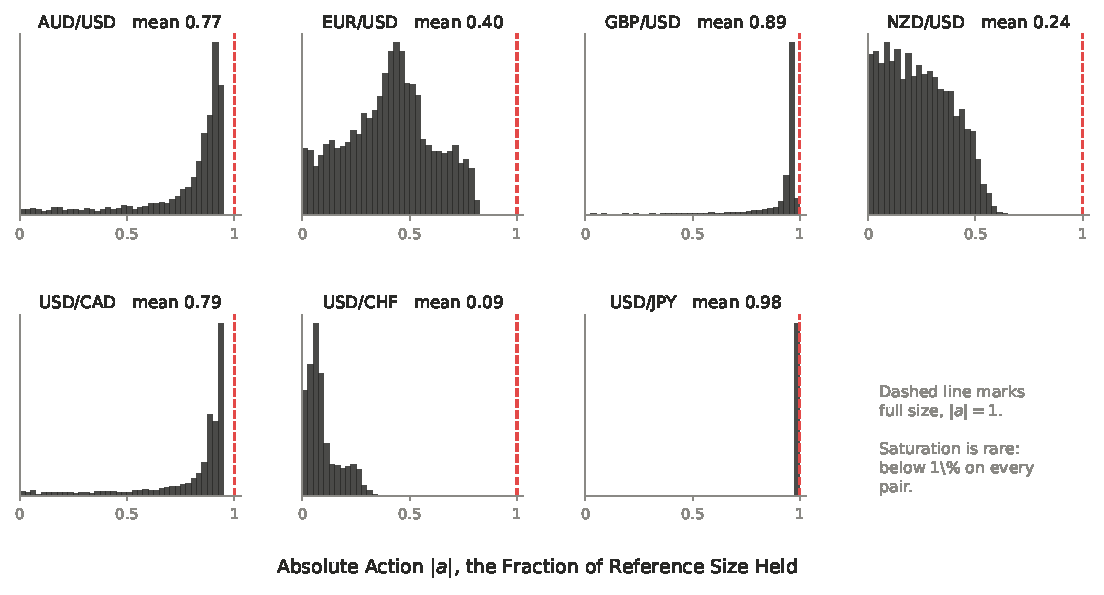
\includegraphics[width=\textwidth]{Images/ActionDistribution.pdf}
\caption{Distribution of the absolute action across the evaluation window. The dashed line marks full size. If the agents had reduced the continuous action to a discrete one, these histograms would be concentrated against that line; instead the mass sits across the interior of the range.}
\label{Figure:ActionDistribution}
\end{figure}

The action does not saturate. Fewer than one percent of decisions on any pair sit above $|a| = 0.98$, and on six of the seven pairs the figure is zero to one decimal place. The mean absolute action ranges from $0.09$ on USD/CHF to $0.98$ on USD/JPY, so the agents settled on very different operating sizes from the same design and the same reference risk.

That spread is itself informative. USD/CHF holds roughly a tenth of the size available to it, which is why its maximum drawdown is $8.2\%$ while its Sharpe ratio is the highest in the set: it found a small edge and sized it accordingly rather than pressing it. NZD/USD, at $0.24$, behaves similarly. USD/JPY sits at the opposite extreme with $0.98$, which is the numerical signature of the failure described in Section~\ref{Subsection:NegativeResult}: an agent that always holds full size in one direction has stopped making a sizing decision at all.

The sizing is adaptive in a second sense that the histogram does not show. The reference size itself is inversely proportional to the average true range, so a constant action produces a smaller position when volatility rises. The action and the volatility scaling compose, and the position actually held is the product of the two.

\subsubsection{Direction, Size and Outcome Together}

Figure~\ref{Figure:DecisionAnatomy} follows EUR/USD through three years, showing the price, the action the agent emitted, the position it held as a result, and the equity that followed.

\begin{figure}[htb!]
\centering
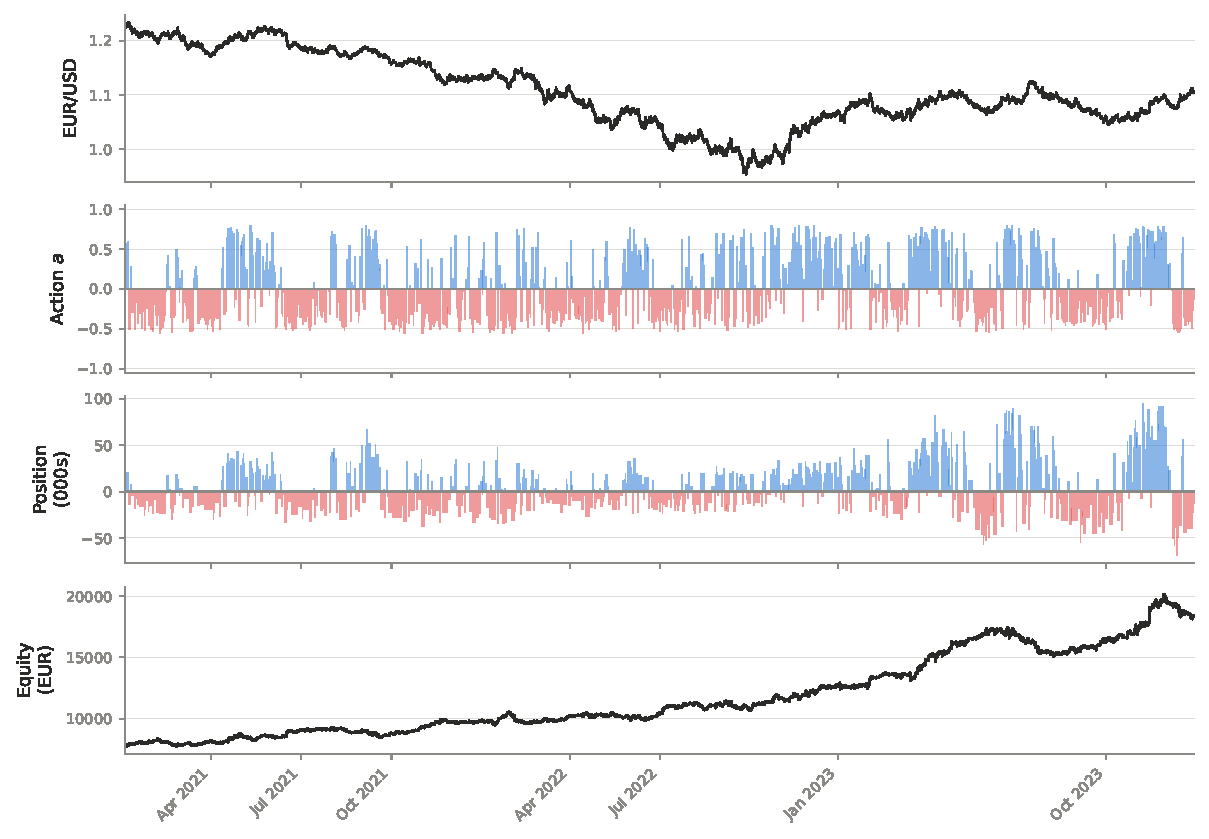
\includegraphics[width=\textwidth]{Images/DecisionAnatomy.pdf}
\caption{EUR/USD from 2021 to 2024. From top: the price; the action, positive for long and negative for short; the resulting net position in thousands of units; and account equity. The action changes sign well before the position does, because a change is only acted on when it exceeds the threshold of Equation~\ref{Equation:Hysteresis}.}
\label{Figure:DecisionAnatomy}
\end{figure}

Three behaviours are visible. The action moves continuously rather than switching between fixed levels, and its magnitude varies as much as its sign. The position follows the action but in coarser steps, because the rebalance threshold suppresses small adjustments; long stretches of constant position correspond to periods where the agent kept revising its target by less than the threshold. And the sign changes are not frequent: over a three-year window the agent reverses direction a few dozen times, which is consistent with the daily decision cadence rather than with an agent reacting to every bar it observes.

\subsubsection{Trend Identification and Reversal}

The clearest illustration of the agents holding a position through a sustained move is GBP/USD in the second half of 2022, shown in Figure~\ref{Figure:TrendRide}. Sterling fell from $1.22$ to below $1.04$ over roughly ten weeks, a decline of more than fifteen percent, with the sharpest part following the United Kingdom fiscal announcement of late September.

\begin{figure}[htb!]
\centering
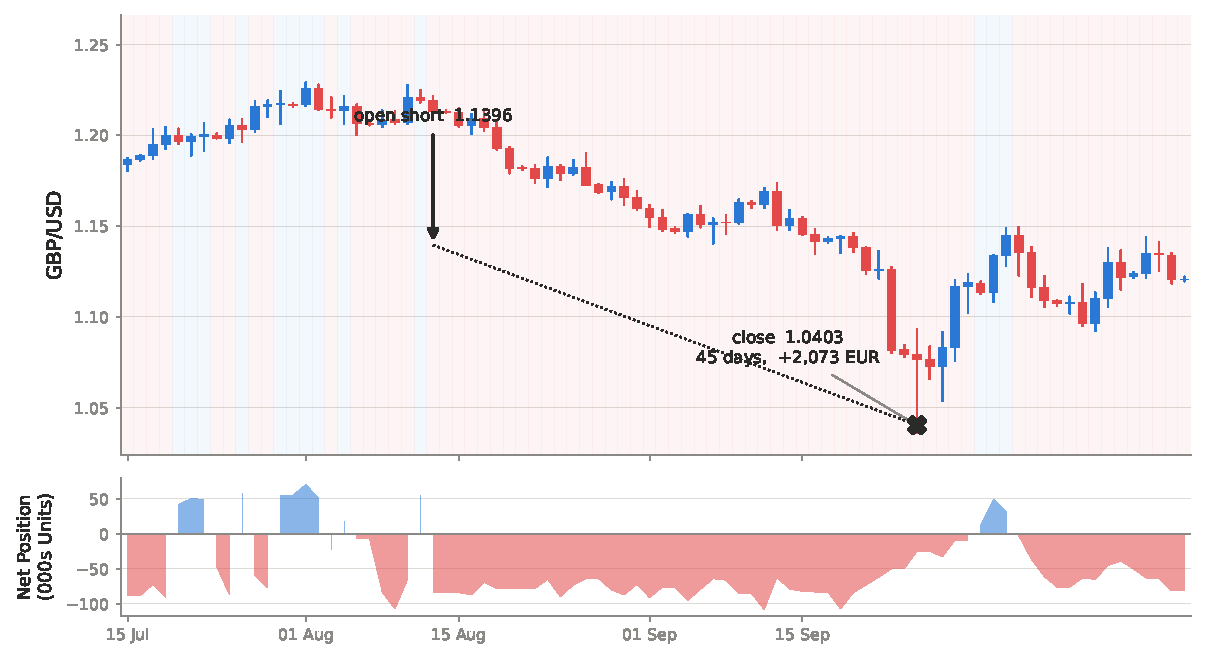
\includegraphics[width=\textwidth]{Images/TrendRide.pdf}
\caption{GBP/USD from mid-July to mid-October 2022. Background shading marks the direction of the net position, red for short and blue for long. The lower pane gives the size of that position. The annotated trade is the single most profitable position of the eleven years on this pair.}
\label{Figure:TrendRide}
\end{figure}

The agent was short for almost the entire decline. It held short exposure of between fifty and one hundred thousand units through the fall, added to it as the move developed, and reduced it into the low. The annotated position was opened at $1.1396$ on 12 August and closed at $1.0403$ on 26 September, forty-five days later, for a net profit of $2\,073$ euros after costs. It is the largest single position of the eleven years on this pair.

Two details are worth pointing out because they show discrimination rather than luck. The agent was briefly long at the end of July, at the local high before the decline began, and it was long again in the days immediately after the bottom, both times at small size. It did not hold the short indefinitely. Once the price recovered above $1.12$ in early October the position was reduced and then reversed, which is the behaviour of an agent responding to the state it observes rather than one committed to a direction.

\subsubsection{Holding Periods and Two-Sided Exposure}

Table~\ref{Tables:Behaviour} gives the trading statistics for each pair and Figure~\ref{Figure:HoldingBehaviour} shows two of them directly. Median holding periods run from four days on EUR/USD to nearly thirteen on GBP/USD, with the longest individual positions measured in months. These are swing traders, not scalpers, which is what the daily decision cadence of Section~\ref{Subsection:ExperimentalProcedure} was intended to produce.

\begin{figure}[htb!]
\centering
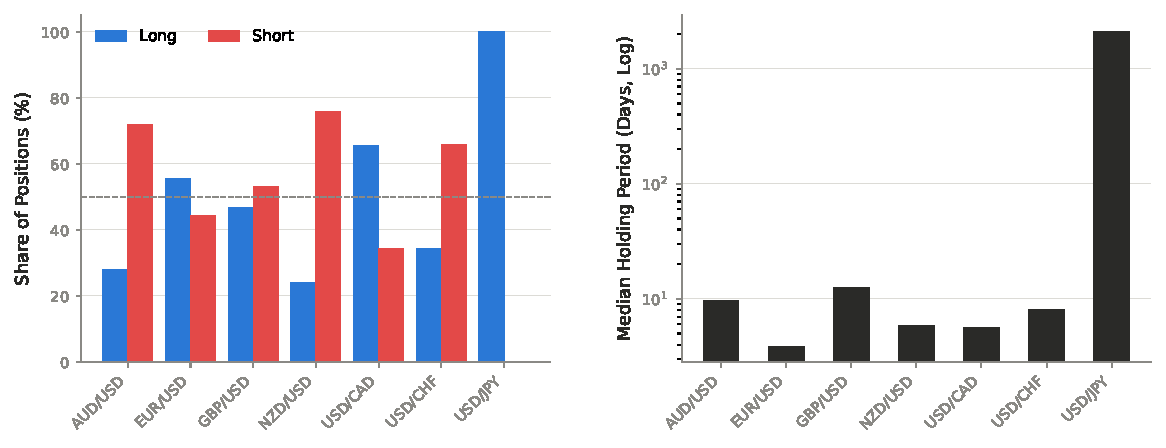
\includegraphics[width=\textwidth]{Images/HoldingBehaviour.pdf}
\caption{Left: the share of positions taken long and short. Right: the median holding period in days, on a logarithmic scale. USD/JPY is long in every position it takes and holds for years, which places it off the scale of the other six.}
\label{Figure:HoldingBehaviour}
\end{figure}

The long and short shares differ substantially between pairs, from $24\%$ long on NZD/USD to $66\%$ on USD/CAD, with EUR/USD and GBP/USD close to balanced. None of the six working agents is one-sided, which is a consequence of the design rather than an accident: the eligibility test of Section~\ref{Subsection:ExperimentalProcedure} rejected any episode whose weaker side fell below a threshold, so a one-sided policy could not be selected however profitable it looked. USD/JPY is the exception at $100\%$ long, and it is the exception precisely because that gate could not be satisfied on that pair by any of the $448$ seeds that were tried.

\subsubsection{Where the Edge Comes From}

One statistic in Table~\ref{Tables:Behaviour} is worth isolating. The win rate, the fraction of positions closed at a profit, lies between $49.8\%$ and $55.0\%$ across the seven pairs. Six of the seven are within three points of a coin flip, and the best model in the set by every risk measure, USD/CHF, has the lowest win rate of all at $49.8\%$.

The agents are therefore not profitable because they are right more often than they are wrong. They are profitable because of what they do with a position once it is open: the size held when the position moves favourably is larger than the size held when it does not, and positions that work are held for longer than positions that do not. That is what a continuous action buys, and it is not available to an agent that can only choose a direction. It also explains why USD/CHF can be the strongest model in the set while being wrong slightly more often than a coin: it is small and patient, and the few positions it holds at size are the ones that worked.

\subsubsection{What the Trading Costs}

Because the engine charges the spread quoted at each fill and a real commission schedule, the difference between what the policies earned and what the account kept can be measured rather than estimated.

The commission is recorded directly on every trade. The spread is not, because it is paid inside each fill rather than deducted after it: a buy is filled at the ask and a sell at the bid, so the cost is already embedded in the entry and exit prices. It can nonetheless be recovered exactly, because the two charges scale in the same way. Commission is levied at $3.5$ points per side, seven points for a round turn, and the spread is crossed once per round turn. Both are proportional to the traded volume and both are converted into the account currency at the same rate, so for any position

\begin{equation}
C_{spread} = \left| C_{commission} \right| \cdot \frac{s}{7}
\label{Equation:SpreadRecovery}
\end{equation}

where $s$ is the spread in points at the moment of the trade. Applying Equation~\ref{Equation:SpreadRecovery} to every position, with $s$ taken from the recorded quotes for the month in which the position was opened, gives Table~\ref{Tables:Costs}.

\begin{table}[htb!]
\centering
\footnotesize
\begin{tabular}{@{}lrrrrrr@{}}
\toprule
\textbf{Pair} & \textbf{Before Costs} & \textbf{Spread} & \textbf{Commission} & \textbf{Net} & \textbf{Cost Share} & \textbf{Mean Spread} \\
\midrule
AUD/USD & 11,851 & $-1,162$ & $-2,200$ & 8,488 & 28.4\% & 3.70 pts \\
EUR/USD & 9,372 & $-638$ & $-1,669$ & 7,064 & 24.6\% & 2.68 pts \\
GBP/USD & 19,086 & $-2,456$ & $-3,168$ & 13,462 & 29.5\% & 5.43 pts \\
NZD/USD & 8,552 & $-1,238$ & $-1,424$ & 5,890 & \textbf{31.1\%} & 6.09 pts \\
USD/CAD & 28,272 & $-2,695$ & $-3,432$ & 22,145 & 21.7\% & 5.50 pts \\
USD/CHF & 5,735 & $-148$ & $-130$ & 5,457 & \textbf{4.8\%} & 7.93 pts \\
USD/JPY & 2,172 & $-411$ & $-155$ & 1,606 & 26.1\% & 18.53 pts \\
\midrule
\textbf{Total} & \textbf{85,039} & $\mathbf{-8,748}$ & $\mathbf{-12,179}$ & \textbf{64,112} & \textbf{24.6\%} & --- \\
\bottomrule
\end{tabular}
\caption{What the seven agents earned before costs and what they kept, in euros. Cost share is the spread and commission together as a fraction of profit before costs. The mean spread column is the commission-weighted average spread paid, in points, which differs from the pair's average spread because it weights the moments the agent actually traded.}
\label{Tables:Costs}
\end{table}

The seven agents earned $85\,039$ euros before costs and kept $64\,112$. Of the difference, $8\,748$ euros went to the spread and $12\,179$ to commission, so \textbf{costs consumed $24.6\%$ of trading profit}. Commission is the larger of the two charges here, which is a consequence of trading a raw-spread account: the spread is narrow by design and the broker recovers its margin explicitly instead. On an account quoting wider spreads with no commission, the same trades would have paid a similar total in a different proportion.

The swap column is absent from Table~\ref{Tables:Costs} because it is zero on every pair. On a swap-free account no overnight financing is charged, so that is the exact figure rather than an approximation, and it matters at this holding horizon: agents holding positions for a median of four to thirteen days would otherwise pay financing on several hundred nights each.

The variation between pairs follows turnover almost exactly, and it is large. USD/CHF takes $220$ positions and surrenders $4.8\%$ of its pre-cost profit, keeping more than nineteen euros in twenty. NZD/USD surrenders $31.1\%$ and GBP/USD $29.5\%$. The same quality of policy therefore delivers very different net results at different trading frequencies, which is why the selection criteria of Section~\ref{Subsection:ExperimentalProcedure} reward long holding periods directly rather than trusting the return figure to account for them, and why the rebalance threshold of Equation~\ref{Equation:Hysteresis} contributes as much as Table~\ref{Tables:Deployment} indicates.

One consequence deserves emphasis because it bears on how the rest of this section should be read. Every return quoted in this work is net of both charges. A study reporting the same policies on bar closes with no spread and no commission would have reported the pre-cost column of Table~\ref{Tables:Costs}, which is a third larger, and it would have been describing a strategy that no account could have traded.

Recovering the spread through Equation~\ref{Equation:SpreadRecovery} works but is indirect, and it relies on the commission being non-zero. The engine computes the spread charge internally when it opens a position and does not currently carry it into the exported trade record as its own field. Recording it there, alongside commission and swap, is a straightforward improvement and is noted in Section~\ref{Subsection:FutureWork}.